\documentclass{homework}

\newcommand{\var}{\mathrm{Var}}
\title{Homework 5}

\begin{document}
    \maketitle

    \problem
    % TODO P1: show 0 quadratic variation of deterministic function

    \problem
    \begin{proof}
        Since
        \[\begin{aligned}
            R_N&=\sum_{i=0}^{N-1}\Delta Z_i(W_{t_{i+1}}-W_{t_i})\\
            &=\sum_{i=0}^{N-1}\big(2W_{t_i^*}-(W_{t_{i_1}}+W_{t_i})
              \big)(W_{t_{i+1}}-W_{t_i})\\ 
            &=2\sum_{i=0}^{N-1}W_{t^*_i}(W_{t_{i+1}}-W_{t_i})
              -\sum_{i=0}^{N-1}(W_{t_{i+1}}^2-W_{t_i}^2)\\
        \end{aligned}\]
        of which the fisrt term is the Stratonovich integral\sidenote{%
        It is a Riemann sum of Stratonovich integral,
        to be more rigorous.}, namely,
        \[\sum_{i=0}^{N-1}W_{t_i^*}(W_{t_{i+1}}-W_{t_i})\to\frac{W_T^2}{2}
        \text{ m.s. }(N\to\infty)\]
        then we have that
        \[R_N\to 0\text{ m.s.}\]
        as
        \[\sum_{i=0}^{N-1}(W_{t_{i+1}}^2-W_{t_i}^2)=W_T^2-W_0^2=W_T^2\]
    \end{proof}

    \problem
    Denote
    \[I_N=\sum_{i=0}^{N-1}W_{t_i^*}(W_{t_{i+1}}-W_{t_i})\]
    then to avoid the overlap between interval $[0,t_i^*]$ and $[t_i,t_{i+1}]$
    for independence consideration, do the decomposition,
    \[\begin{aligned}
        I_N&=\sum_{i=0}^{N-1}W_{t_i^*}(W_{t_{i+1}}-W_{t_i^*})
        +W_{t_i^*}(W_{t_i^*}-W_{t_i})\\
    \end{aligned}\]
    and we split $W_{t_i^*}$ again in the last term,
    \[\begin{aligned}
        I_N&=\sum_{i=0}^{N-1}W_{t_i^*}(W_{t_{i+1}}-W_{t_i^*})
        +(W_{t_i^*}-W_{t_i})^2+W_{t_i}(W_{t_i^*}-W_{t_i})\\
        &=\sum_{i=0}^{N-1}\left(W_{t_i^*}(W_{t_{i+1}}-W_{t_i^*})
            +W_{t_i}(W_{t_i^*}-W_{t_i})\right)
          +\sum_{i=0}^{N-1}(W_{t_i^*}-W_{t_i})^2
    \end{aligned}\]
    Now take a close look at the first term, and it is easy to
    see that it is the It\^o  integral actually, i.e., consider
    the following partition\sidenote{If $\lambda=0\text{ or }1$,
    then it is not a partition. But it is a degenerated case actually,
    namely a partition with $N$ slices, so it is ok as well.} of $[0,T]$,
    \[0=t_0<t_0^*<t_1<t_1^*<\cdots<t_{N-1}<t_{N-1}^*<t_N=T\]
    and denote 
    \[\tilde t_i=\begin{cases}
        t_k&,i=2k\\
        t_k^*&,i=2k+1
    \end{cases}\]
    then $0=\tilde t_0<\tilde t_1<\cdots<\tilde t_{2N}=T$ is the finer
    partition, thus
    \[\sum_{i=0}^{N-1}\left(W_{t_i^*}(W_{t_{i+1}}-W_{t_i^*})
            +W_{t_i}(W_{t_i^*}-W_{t_i})\right)
    =\sum_{i=0}^{2N}W_{\tilde t_i}(W_{\tilde t_{i+1}}-W_{\tilde t_i})\]
    which will converge to $(W_T^2-T)/2$ in m.s. as we leant
    in class.

    As for the latter term, we obtained its variance as
    \[\var\left(\sum_{i=0}^{N-1}(W_{t_i^*}-W_{t_i})^2\right)
    =\sum_{i=0}^{N-1}\var\left((W_{t_i^*}-W_{t_i})^2\right)
    =\sum_{i=0}^{N-1}2(t_i^*-t_i)^2\]
    by the independence of each term and formula,
    \[\var(X^2)=2\sigma^4\text{ if }X\sim\mathcal N(\mu,\sigma^2)\]
    If we denote $\tau=\sup_{0\leq i\leq N-1}(t_{i+1}-t_i)$ to describe
    the mesh, then $N\to\infty$ is equivalent to $\tau\to 0^+$, and
    \[\begin{aligned}
        \var\left(\sum_{i=0}^{N-1}(W_{t_i^*}-W_{t_i})^2\right)
    &\leq 2\sum_{i=0}^{N-1}(t_{i+1}-t_i)^2\\
    &\leq 2\tau\sum_{i=0}^{N-1}t_{i+1}-t_i\\
    &=2T\tau\to 0\quad(\tau\to 0^+)
    \end{aligned}\]
    and the expectation
    \[\begin{aligned}
        E\left(\sum_{i=0}^{N-1}(W_{t_i^*}-W_{t_i})^2\right)
        &=\sum_{i=0}^{N-1}t_i^*-t_i\\
        &=\sum_{i=0}^{N-1}(1-\lambda)t_i+\lambda t_{i+1}-t_i\\
        &=\lambda\sum_{i=0}^{N-1}t_{i+1}-t_{i}\\
        &=\lambda T
    \end{aligned}\]
    therefore,
    \[\sum_{i=0}^{N-1}(W_{t_i^*}-W_{t_i})^2\to\lambda T
    \text{ in m.s.}\]
    It follows that
    \[I_N\to \frac{W_T^2}{2}+\left(\lambda-\frac{1}{2}\right)T
    \quad(N\to\infty)\]
    in m.s., i.e.,
    \[\int_0^TW_t\diamond\diff W_t=
    \frac{W_T^2}{2}+\left(\lambda-\frac{1}{2}\right)T\]

    \problem
    % TODO ti*(Wti - Wt(i+1))^2

    \problem
    See \cref{fig:numerical solution}.
    \begin{figure}[h]
        \centering
        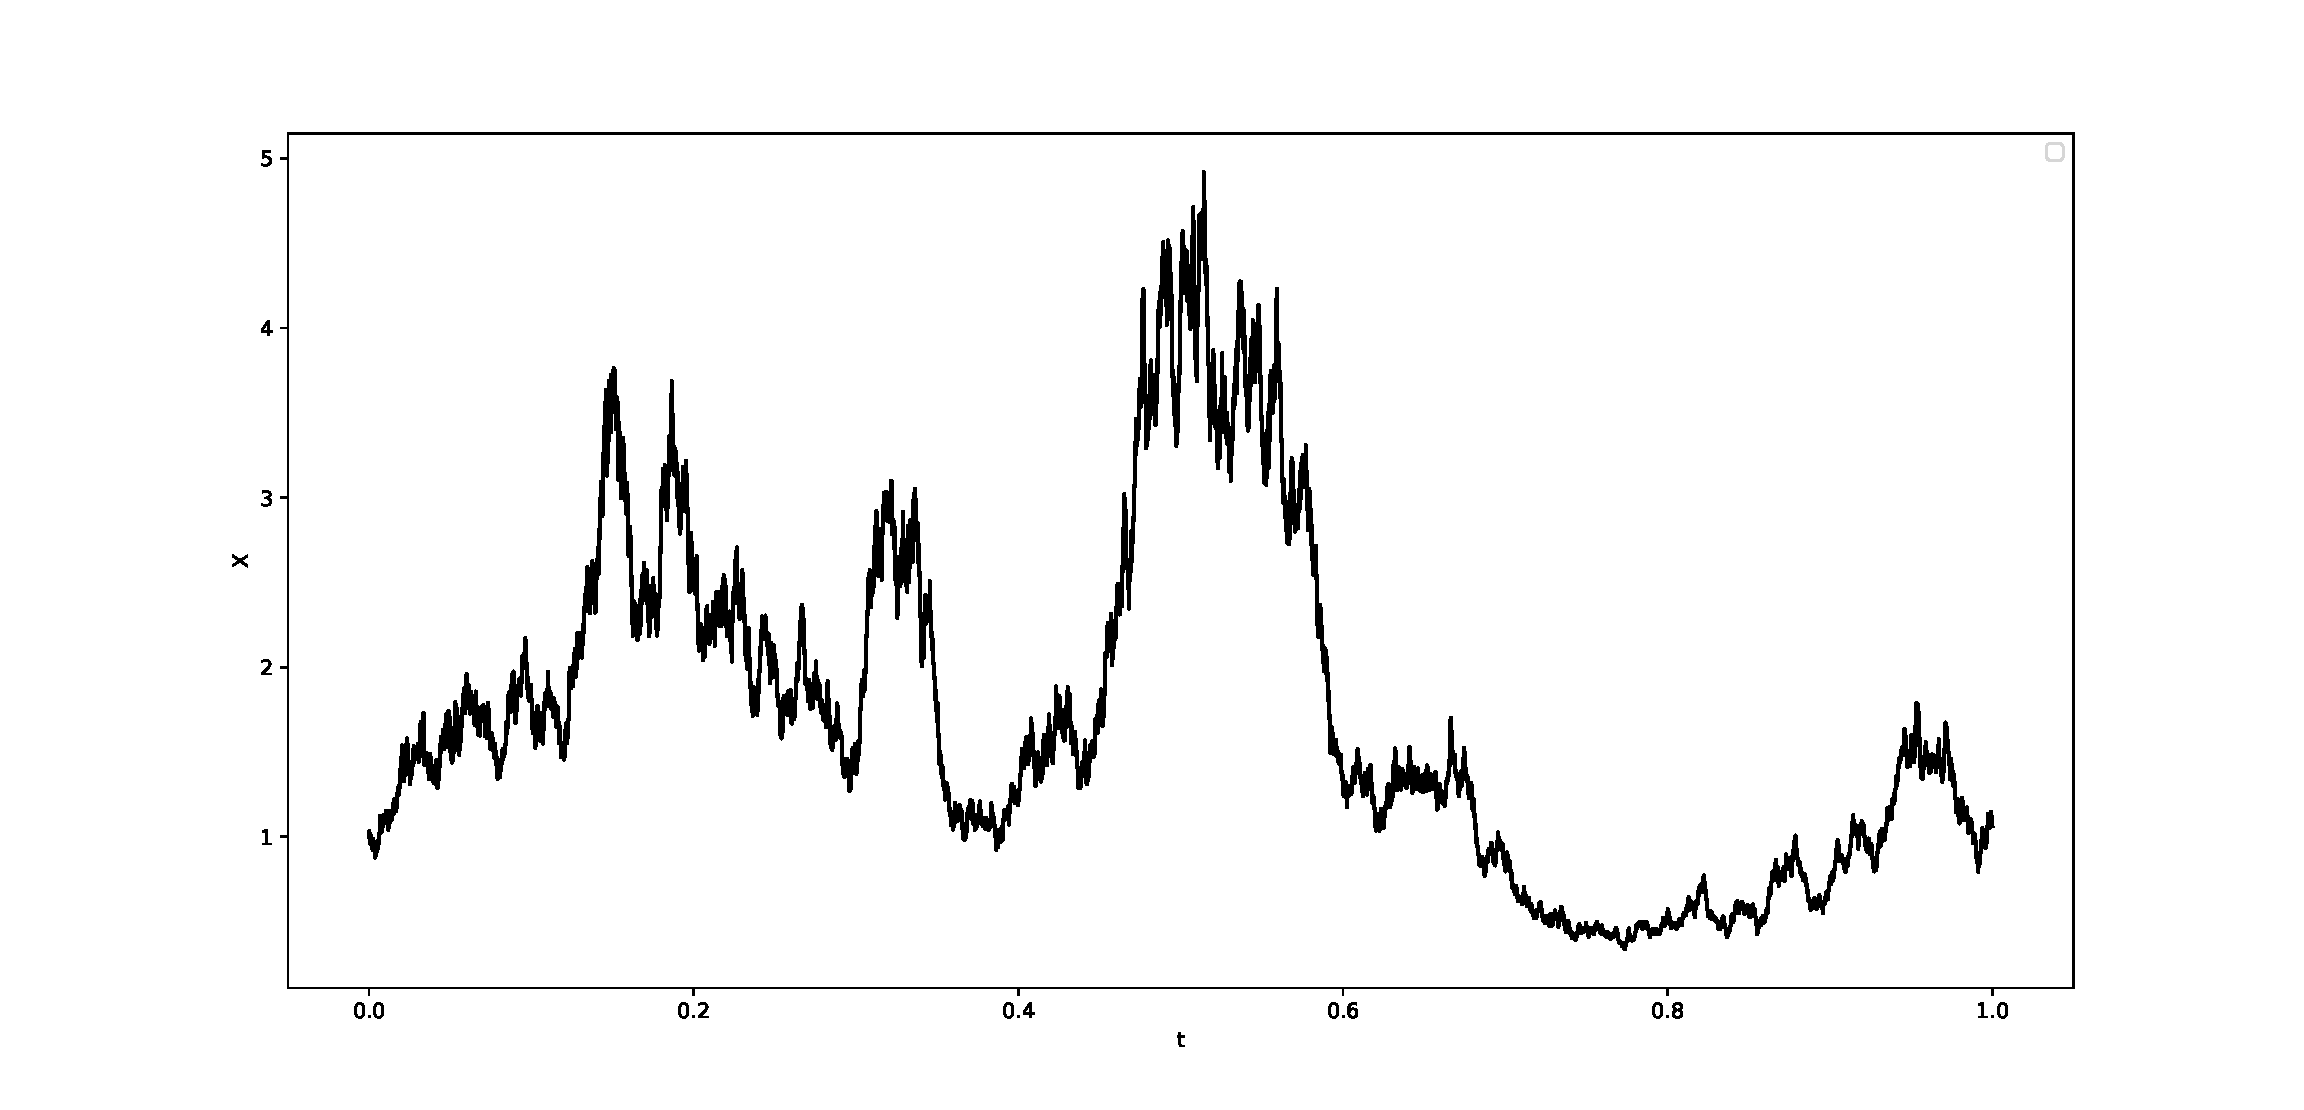
\includegraphics[width=\linewidth]{solution}
        \caption{Numerical Solution}
        \label{fig:numerical solution}
    \end{figure}

    \appendix
    \section{Python Code for Numerical Solution}
    \lstinputlisting[language=Python]{numerical.py}
\end{document}